\documentclass[a4paper,12pt]{article} 
\usepackage[french]{babel}
\usepackage[utf8]{inputenc}
\usepackage{answers}

\usepackage{hyperref}

\usepackage[table,xcdraw]{xcolor}
\usepackage{listings}
\definecolor{ForestGreen}{RGB}{34,139,34}

\usepackage{multicol}

\usepackage{enumitem}

\newcommand{\py}{\lstinline{Python} }

%%%%%%%%%%%%%%%%%%%%%%%%%%%%%%%% CONSTANTES %%%%%%%%%%%%%%%%%%%%%%%%%%%%%%%%%%%
\newcommand{\numero}{1}                                    %Numéro de la série -1


\definecolor{backcolour}{rgb}{0.95,0.95,0.92}

\lstset{%
	language         = Python,
	backgroundcolor  = \color{backcolour},
	basicstyle       = \ttfamily, % \upshape\ttfamily,
	keywordstyle     = \bfseries\color{blue}, %\bfseries,
	stringstyle      = \color{magenta},
	commentstyle     = \color{ForestGreen},
	alsoletter = > ,
	morekeywords = {>>>,as,assert,False,None, nonlocal,True, with,yield},
	showstringspaces = false,
	numbers=left,
	stepnumber=1,
	literate={à}{{\`{a}}}1 {é}{{\'e}}1 {è}{{\`{e}}}1 {ê}{{\^{e}}}1 {ç}{{\c{c}}}1 {Ç}{{\c{C}}}1,
}

\newcommand{\itemb}[1]{\item \textbf{#1}}

\usepackage{fancyhdr}  %package pour en-tetes et pied de pages
\usepackage{sectsty} % Permet de faire des modifications de police dans diverses sections des "headings" (cf. modif presentation de la page)
\pagestyle{fancy}       %Style pour en-tetes et pieds de pages
\fancyhead[CO,CE]{\sc Série 1\hspace{0.5mm}}
\fancyhead[RO,LE]{Collège Sismondi}  % LaTeX/TEX define \strut to be an invisible box of width zero that extends just enough above and below the baseline. Cela permet d'augementer légèrement la taille en bas de la box de manière à ce qu'elle soit collée à la ligne.
\fancyhead[LO,RE]{\small\ \textsl{1\textsuperscript{er} année - Informatique}}
\fancyfoot[RO,LE]{2021 - 2022}
\fancyfoot[LO,RE]{\small M.Schiess }
\fancyfoot[CO,CE]{\thepage}

\fancyhfoffset[l]{1.2cm} % le "l" en paramètre permet d'indiquer qu'on ne veut modifier que la marge à gauche.
\renewcommand{\headrule}{{%
		\hrule \headwidth \headrulewidth \vskip-\headrulewidth}}
\renewcommand\footrulewidth{\headrulewidth}
\renewcommand{\footrule}{{%
		\vskip-\footruleskip\vskip-\footrulewidth
		\hrule \headwidth \footrulewidth\vskip\footruleskip}}

\usepackage{tikz}
%-------------------------------------------------------------------------------
%---- Eclairage : en encadré sur fond jaune avec symbôle "ampoule" à gauche ----
%-------------------------------------------------------------------------------
\definecolor{coleclairage}{RGB}{255 , 221 , 156}
\definecolor{contoureclairage}{RGB}{255 , 192 , 0}
\newenvironment{eclairage}
{
	\begin{center}%
		\begin{tikzpicture}%
			\node[rectangle, draw=contoureclairage, top color=coleclairage!50, bottom color=coleclairage!140, rounded corners=5pt, inner xsep=5pt, inner ysep=6pt, outer ysep=10pt]\bgroup                     
			\begin{minipage}{0.98\linewidth}
				\begin{minipage}{0.08\linewidth}\centerline{
\includegraphics[scale=1]{../../theorie/Images/Symbole_eclairage.png}}\end{minipage}
				\begin{minipage}{0.89\linewidth}\itshape\footnotesize
				}
				{                		
				\end{minipage}
			\end{minipage}\egroup;%
		\end{tikzpicture}%
	\end{center}%
}

%-------------------------------------------------------------------------------
%---- apprendre : en encadré sur fond jaune avec symbôle "ampoule" à gauche ----
%-------------------------------------------------------------------------------
\definecolor{colapprendre}{RGB}{50,205,50}
\definecolor{contourapprendre}{RGB}{34,139,34}
\newenvironment{apprendre}
{
	\begin{center}%
		\begin{tikzpicture}%
			\node[rectangle, draw=contourapprendre, top color=colapprendre!10, bottom color=colapprendre!50, rounded corners=5pt, inner xsep=5pt, inner ysep=6pt, outer ysep=10pt]\bgroup                     
			\begin{minipage}{0.98\linewidth}
				\begin{minipage}{0.08\linewidth}\centerline{
\includegraphics[width=30px]{../../theorie/Images/Symbole_learn.png}}\end{minipage}
				\begin{minipage}{0.89\linewidth}\itshape\footnotesize
				}
				{                		
				\end{minipage}
			\end{minipage}\egroup;%
		\end{tikzpicture}%
	\end{center}%
}


%-----------------------------------------------------------------
%---- Modification présentation de la page: marges de la page ----
%-----------------------------------------------------------------
%\addtolength{\hoffset}{-1in}              % 1
%\addtolength{\voffset}{-1in}              % 2
\addtolength{\oddsidemargin}{-0.1 in} % 3
\addtolength{\evensidemargin}{-1in} % 3
\addtolength{\topmargin}{-1in}       % 4
\addtolength{\headheight}{6pt}       % 5
%\addtolength{\headsep}{-0.2cm}           % 6
\setlength{\textheight}{26cm}    % 7
\setlength{\textwidth}{16.5cm}      % 8
\addtolength{\marginparsep}{0pt}      % 9
\setlength{\marginparwidth}{0pt}   % 10
\addtolength{\footskip}{-1mm}           %11

\setlength{\parindent}{0em}% pas d'indentation


% Customiser le nom des sections
\usepackage{titlesec}
\titleformat{\section}[hang]{\Large \bfseries}{Série \thesection:\ }{0pt}{}

\renewcommand{\familydefault}{\sfdefault} % pour avoir des polices san serif

\newtheorem{Exc}{Exercice}
\Newassociation{correction}{Soln}{mycor}
\renewcommand{\Solnlabel}[1]{\bfseries Ex #1 }
\def\exo#1{%
	\futurelet\testchar\MaybeOptArgmyexoo}
\def\MaybeOptArgmyexoo{
	\ifx[\testchar \let\next\OptArgmyexoo
	\else \let\next\NoOptArgmyexoo \fi \next}
\def\OptArgmyexoo[#1]{%
	\begin{Exc}[#1]\normalfont}
	\def\NoOptArgmyexoo{%
		\begin{Exc}\normalfont}
		\newcommand{\finexo}{\end{Exc} \vspace{3mm}}
	\newcommand{\flag}[1]{}
	\newcommand{\entete}[1]

\newcommand{\getexocompteur}{{\the\numexpr \arabic{Exc}  \relax}}	
	
\newcommand{\eexo}{\vspace{5mm}} % espace pour séparer les exercices

\begin{document}
%		\title{\vspace{-3cm}Série 1}
%		\date{\vspace{-2cm}}
%		\maketitle

\fancyhead[CO,CE]{\sc Série \arabic{section} \hspace{0.5mm}}

\setcounter{section}{\numero}
\section{Représentation de textes et d'images }				
\Opensolutionfile{mycor}[cor_01]

\exo{}[Coder un texte en binaire, avec corrigé détaillé]  ~\\ 
	Trouver la représentation binaire en ASCII du texte « Je pense, donc je suis. » 

	\begin{correction}
		~\\ 
On cherche la table des codes ASCII sur le Web de manière à traduire le texte, caractère par
caractère : 74, 101, 32, 112, 101, 110, 115, 101, 44, 32, 100, 111, 110, 99, 32, 106, 101, 32,
115, 117, 105, 115, 46. On exprime ensuite chacun de ces nombres en binaire sur huit bits :\\
01001010 01100101 00100000 01110000 01100101 01101110 01110011 01100101 00101100\\
00100000 01100100 01101111 01101110 01100011 00100000 01101010 01100101 00100000\\
01110011 01110101 01101001 01110011 00101110.\\
 
	\end{correction}
\finexo

\exo{}[Coder un texte en binaire]  ~\\ 
Trouver la représentation binaire en ASCII du texte "Cet exercice est un peu fastidieux."
	\begin{correction}
	~\\ 01000011 01100101 01110100 00100000 01100101 01111000 01100101 01110010 01100011\\
	     01101001 01100011 01100101 00100000 01100101 01110011 01110100 00100000 01110101\\
	     01101110 00100000 01110000 01100101 01110101 00100000 01100110 01100001 01110011 \\
	     01110100 01101001 01100100 01101001 01100101 01110101 01111000 00101110
\end{correction}
\finexo

\exo{}  ~\\ 
	Écrire les nombres suivants en base hexadécimal:
	\begin{multicols}{2}
		\begin{enumerate}
			\item $10010010110_{(2)}$
			\item $111110_{(2)}$
			\item  $1000110101110101_{(2)}$
			\item $11110000000011_{(2)}$
		\end{enumerate}
	\end{multicols}
	\begin{correction}
	~\\ \vspace{-7mm}
	\begin{multicols}{2}
		\begin{enumerate}
			\item $496_{(16)}$
			\item $3E_{(16)}$
			\item  $8D75_{(16)}$
			\item $3C03_{(16)}$
		\end{enumerate}
	\end{multicols}
\end{correction}
\finexo

\exo{}[Lire un texte écrit en binaire, avec corrigé détaillé]  ~\\ 
Trouver le texte représenté en ASCII binaire par la suite de bits\\
01000011 00100111 01100101 01110011 01110100 00100000 01100110 01100001  
01100011 01101001 01101100 01100101.
	\begin{correction}
	~\\ 
	On commence par découper la suite de bits en octets : 01000011 00100111 01100101
	01110011 01110100 00100000 01100110 01100001 01100011 01101001 01101100 01100101.\\
	Chaque octet représente un nombre entier : 67, 39, 101, 115, 116, 32, 102, 97, 99, 105, 108,
	101. On cherche ensuite la table des codes ASCII en ligne de manière à traduire chacun de
	ces nombres en une lettre : « C’est facile ».
\end{correction}
\finexo

\exo{}[Lire un texte écrit en binaire]  ~\\ 
Trouver le texte représenté en ASCII binaire par la suite de bits\\
00110000 01110100 01100101 01110100 01110100 00110001.
\begin{correction}
	~\\ 
 « 0tett1 »
\end{correction}
\finexo


\exo{}[Éditeur hexadécimal]  ~\\ 
\begin{enumerate}
	\item Ouvrir l'éditeur de texte "kate", puis créer un fichier texte qui contient le texte « Je pense, donc je suis. ». Sauver le fichier texte sous le nom "ex\_phrase.txt".
	\item Ouvrir le fichier avec un éditeur hexadécimal, par exemple l'éditeur en ligne HexEd (\url{https://hexed.it/}) ou "Okteta" (si installé).
	\item Donner la représentation en hexadécimal du code ASCII du fichier.
\end{enumerate}

\finexo


\exo{}[Nécessité de méta-données]  ~\\ 
	Une image a été codée avec la suite de bits suivante\\
00000000000011111100011000011001000000100100000010010000001001000000100110000110
00111111000000000000

\begin{enumerate}
	\item Pouvez-vous déterminer ce que représente cette image?
	\item Même question mais sachant que cette suite de bits représente une image de dimension 10 x 10.
\end{enumerate}
\begin{correction}
	~\\ 
	\begin{center}
		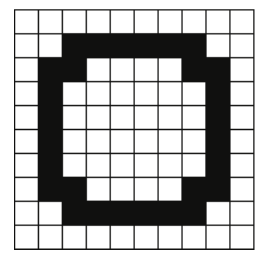
\includegraphics[scale=0.5]{images/img_zero.png}
	\end{center}
	
\end{correction}
\finexo

\newpage

\exo{}[Codage binaire d'image]  ~\\ 
Coder chaque image en utilisant 1 bit par pixel (même codage qu'étudié dans la théorie). Indiquer les dimensions de chaque image
\begin{center}
	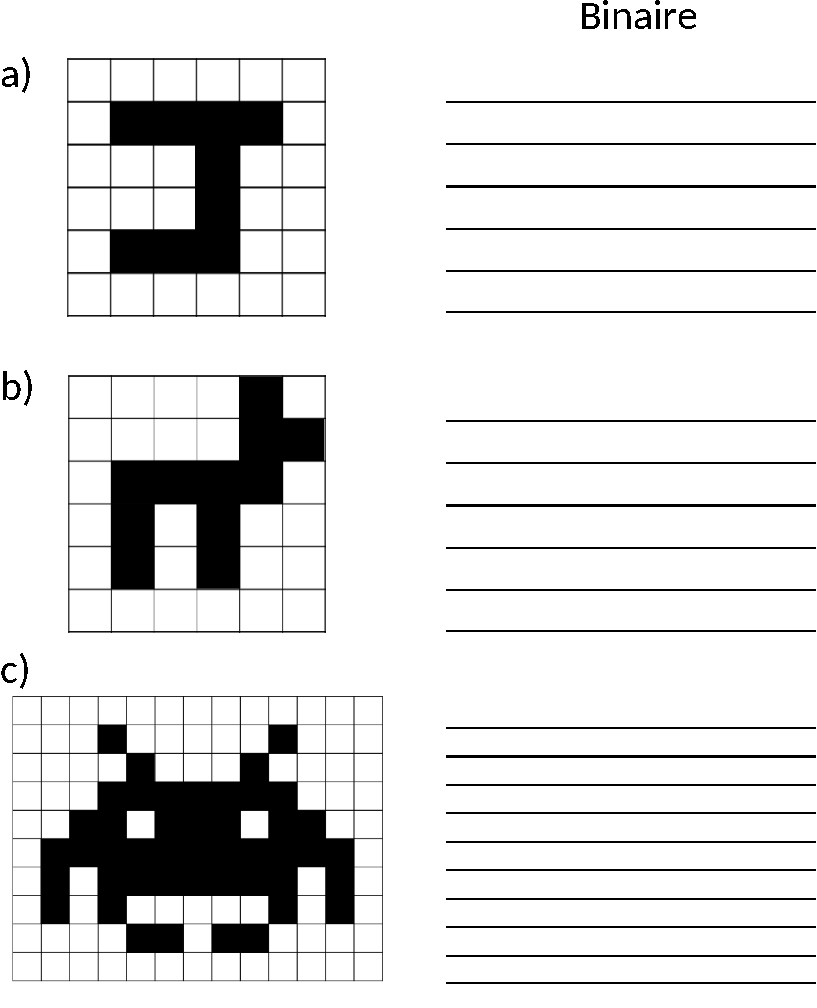
\includegraphics[scale=0.8]{images/exo_image_bin-crop.pdf}
\end{center}
\begin{correction}
	~\\
	\begin{multicols}{2}
		\begin{enumerate}[label=\alph*)]
			\item  0 0 0 0 0 0\\
				   0 1 1 1 1 0\\
				   0 0 0 1 0 0\\
				   0 0 0 1 0 0\\
				   0 1 1 1 0 0\\
				   0 0 0 0 0 0\\
				   
	        \item  0 0 0 0 1 0\\
	               0 0 0 0 1 1\\
	               0 1 1 1 1 0\\
	               0 1 0 1 0 0\\
	               0 1 0 1 0 0\\
	               0 0 0 0 0 0\\
	        \item  0 0 0 0 0 0 0 0 0 0 0 0 0\\
	               0 0 0 1 0 0 0 0 0 1 0 0 0\\
	               0 0 0 0 1 0 0 0 1 0 0 0 0\\
	               0 0 0 1 1 1 1 1 1 1 0 0 0\\
	               0 0 1 1 0 1 1 1 0 1 1 0 0\\
	               0 1 1 1 1 1 1 1 1 1 1 1 0\\
	               0 1 0 1 1 1 1 1 1 1 0 1 0\\
	               0 1 0 1 0 0 0 0 0 1 0 1 0\\
	               0 0 0 0 1 1 0 1 1 0 0 0 0\\
	               0 0 0 0 0 0 0 0 0 0 0 0 0\\
		\end{enumerate}
		\end{multicols} 	
\end{correction}
\finexo

\exo{}[Un autre codage binaire d'image]  ~\\ 
   Un nouvelle représentation d'images en noir et blanc est proposé. Dans ce système chaque ligne est représentée par un suite de nombre qui code l'alternance entre pixel blanc et noir.
   \begin{center}
   	   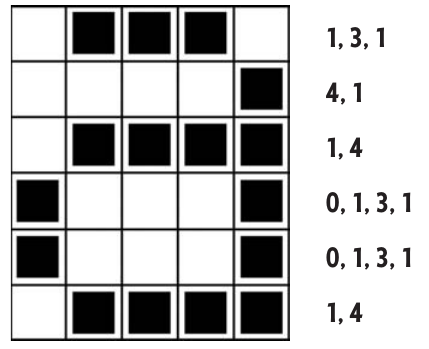
\includegraphics[scale=0.5]{images/exo_code_imgBin_alt.png}
   \end{center}
	L’image ci-dessus nous montre illustre le codage proposé. La première ligne contient un pixel blanc, trois noirs puis un blanc. Ainsi, la première ligne est représentée par 1, 3, 1. Le premier nombre représente toujours le nombre de pixels blancs. Si le premier pixel est noir, la ligne commencera par un 0.\\
	\newpage
	Décoder les image ci-dessous en compétant les grilles de pixels.
	   \begin{center}
		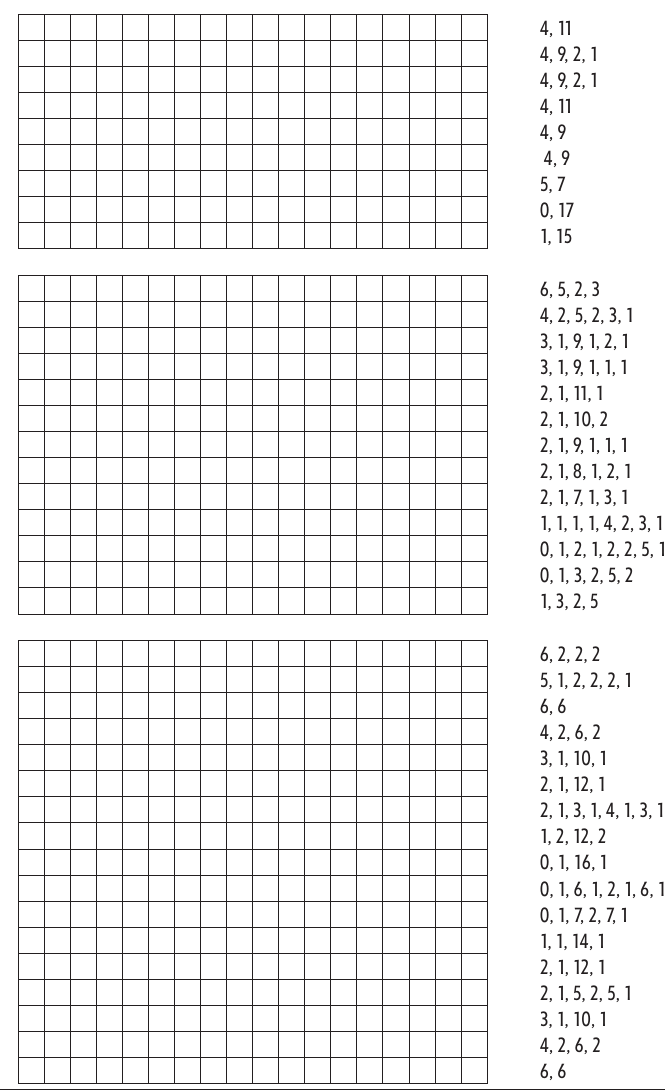
\includegraphics[scale=0.8]{images/decode_exo_code_imgBin_alt.png}
	\end{center}

\begin{correction}
	~\\	   \begin{center}
		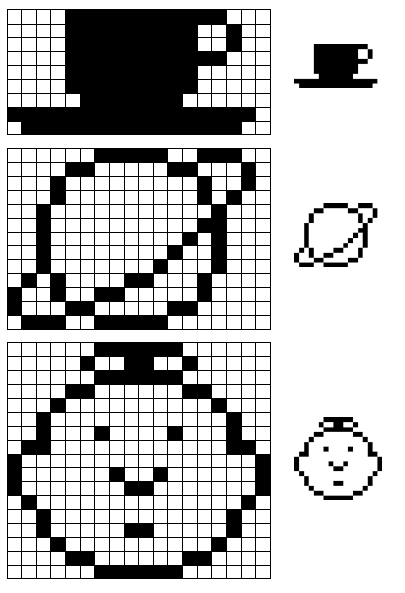
\includegraphics[scale=0.8]{images/corr_exo_code_imgBin_alt.png}
	\end{center}
	
\end{correction}

\finexo

% Solution		
		\newpage
		\setcounter{page}{1}
		\setcounter{section}{\numero}
		\Closesolutionfile{mycor}
		\titleformat{\section}[hang]{\Large \bfseries}{Corrigé Série \thesection:\ }{0pt}{}
		

		\fancyhead[CO,CE]{\sc Corrigé Série \arabic{section} \hspace{0.5mm}}
		\section{}
		\Readsolutionfile{mycor}
	\end{document}